In this section, we use the estimated parameters from the previous section to analyze Model (\ref{model1}) and the effect of the vaccine. Some plausible scenarios are presented, depending on the effectiveness of the vaccine,  as well as the rate of vaccination.

In the first instance, it has been shown that the interest region of the state variables of the system is positively invariant. This implies that any solution with initial conditions within that region will remain within it.

%Let $\Omega=\{(S,E,I_S,I_A,R,D,V)\in \R^{7}_{+}: S+E+I_S+I_A+R+D+V=N\}$. First, note that for this model we have a closed population, which allows the solutions to be bounded superiorly by the total population. 

%On the other hand, to show the positivity of the solutions with initial conditions $(S (0), E (0), I_S (0), I_A (0), R (0), D (0), V (0)) \in \R^{7}_{+}$, we look at the direction of the vector field on the hypercube faces in the direction of each variable in the system. For example, consider a point on the hypercube face where the variable $S = 0$ and look at the behavior of the vector field in the direction of the same variable $S$, to see if the solutions cross the face of the hypercube where we are taking the initial condition. So, notice that if $ S = 0 $, $ S '(t) > 0 $, so the solution points into the hypercube. Similarly, consider an initial condition of the form $ (S, 0, I_S, I_A, R, D, V) $ and note that $ E '(t)> 0 $ for all $ t> 0 $, which implies that the solutions of the system with initial conditions of the form $  (S, 0, I_S, I_A, R, D, V)  $ point towards the interior of the hypercube. Similarly, positivity can be tested for the rest of the variables. With this information, we have the following result.

%\begin{lemma}
%The set  $\Omega=\{(S,E,I_S,I_A,R,D,V)\in \R^{7}_{+}: S+E+I_S+I_A+R+D+V=N\}$ is a positively invariant set for the system (\ref{model1}).
%\end{lemma}
%Continuing with the analysis of our model, it is easy to prove that the disease-free equilibrium is given by the point at $ X_0 \in \Omega $ of the form $X_0=(\frac{(\mu+\delta_V)\bar{N}}{\mu+\delta_V+\lambda_V},0,0,0,0,\frac{\lambda \bar{N}}{\mu+\delta_V+\lambda_V})$. 

Now, using the next-generation matrix method  \cite{Diekmann1990, Van2002}, the basic reproductive number for system (\ref{model1}) is given by


%to calculate it \cite{Diekman, Driessche} we have that the next generation matrix for this model is given by


%\begin{align}\label{NGM1}
%\begin{split}
%\textbf{K}=
%\begin{bmatrix}
%\frac{\delta_E}{(\mu+\delta_E)}\left(\frac{p\beta_S}{\mu+\alpha_S+\mu_S+\lambda_T}\right)(S^*+\epsilon V^*) & \frac{\beta_S (S^*+\epsilon V^*)}{(\mu+\alpha_S+\mu_S+\lambda_T)\bar{N}} & \frac{\beta_A (S^*+\epsilon V^*)}{(\mu+\alpha_A+\mu_A)\bar{N}}\\
%0 & 0 & 0 \\
%0 & 0 & 0  \\
%\end{bmatrix}
%\end{split}
%\end{align}

%where $S^*=\frac{(\mu+\delta_V)\bar{N}}{\mu+\delta_V+\lambda_V}$ and $V^*=\frac{\lambda \bar{N}}{\mu+\delta_V+\lambda_V}$. So, the basic reproduction number for this model is

\begin{equation}\label{Rv}
R_{V}=R_S+R_A
\end{equation}
with

\begin{eqnarray*}
R_S&=&\frac{p\beta_S\delta_E(\mu+\delta_V+(1-\epsilon) \lambda_V)}{(\mu+\delta_E)(\mu+\delta_V+\lambda_V)(\mu+\alpha_S+\mu_S+\lambda_T)}\\ 
 R_A&=&\frac{(1-p)\beta_A\delta_E(\mu+\delta_V+(1-\epsilon) \lambda_V)}{(\mu+\delta_E)(\mu+\delta_V+\lambda_V)(\mu+\alpha_A+\mu_A)}.\nonumber
\end{eqnarray*}
 Note that each sum of $ R_ {V} $ represents the contribution of the symptomatic and asymptomatic infected, respectively, to the spread of the disease.

Now, following the ideas of Alexander et.al. \cite{Alexander2004}, expression for $R_V$ can be rewritten as

\begin{equation}\label{Rv2}
R_{V}=R_0\left(1- \frac{\epsilon \lambda_V}{(\mu+\delta_V+\lambda_V)}\right)
\end{equation}
where $R_0$ is the basic reproduction number of system without vaccine. Note that $\left(1- \frac{\epsilon \lambda_V}{(\mu+\delta_V+\lambda_V)}\right)<1$, Therefore, this factor which saves the parameters corresponding to the application of the vaccine will allow us to modulate the value of $ R_0 $. In the first instance, if $ R_0 <1 $, then $ R_V <1 $. But, if $ R_0> 1 $, we wonder if the application of the vaccine can lower $R_V$ value below 1. In this sense, it is easy to prove that, if

\begin{equation}\label{condition1}
\epsilon>\frac{(R_0-1)(\mu+\delta_V+\lambda_V)}{R_0\lambda_V},
\end{equation}

\noindent it is possible to reduce the value of $ R_V $ below one, of course with the necessary conditions in terms of vaccination. That is, there is a region in the parameter space in which it is possible to reduce the value of $ R_V $ below one, considering adequate efficacy, vaccination rate and duration of the effect of the vaccine. However, if the inequality (\ref{condition1}) is not satisfied, it will not be possible to reduce the value of $ R_V $ below 1.

To illustrate the aforementioned, Figure \ref{figure3} shows the regions where it is possible to reduce the value of $ R_V $. In this case, we set all the system parameters, which are given in table \ref{table1} and with $ \delta_V = 2/365 $, leaving $ \epsilon $ and $ \lambda_V $ free. 

%\begin{figure}[!h]\label{figure3}
%  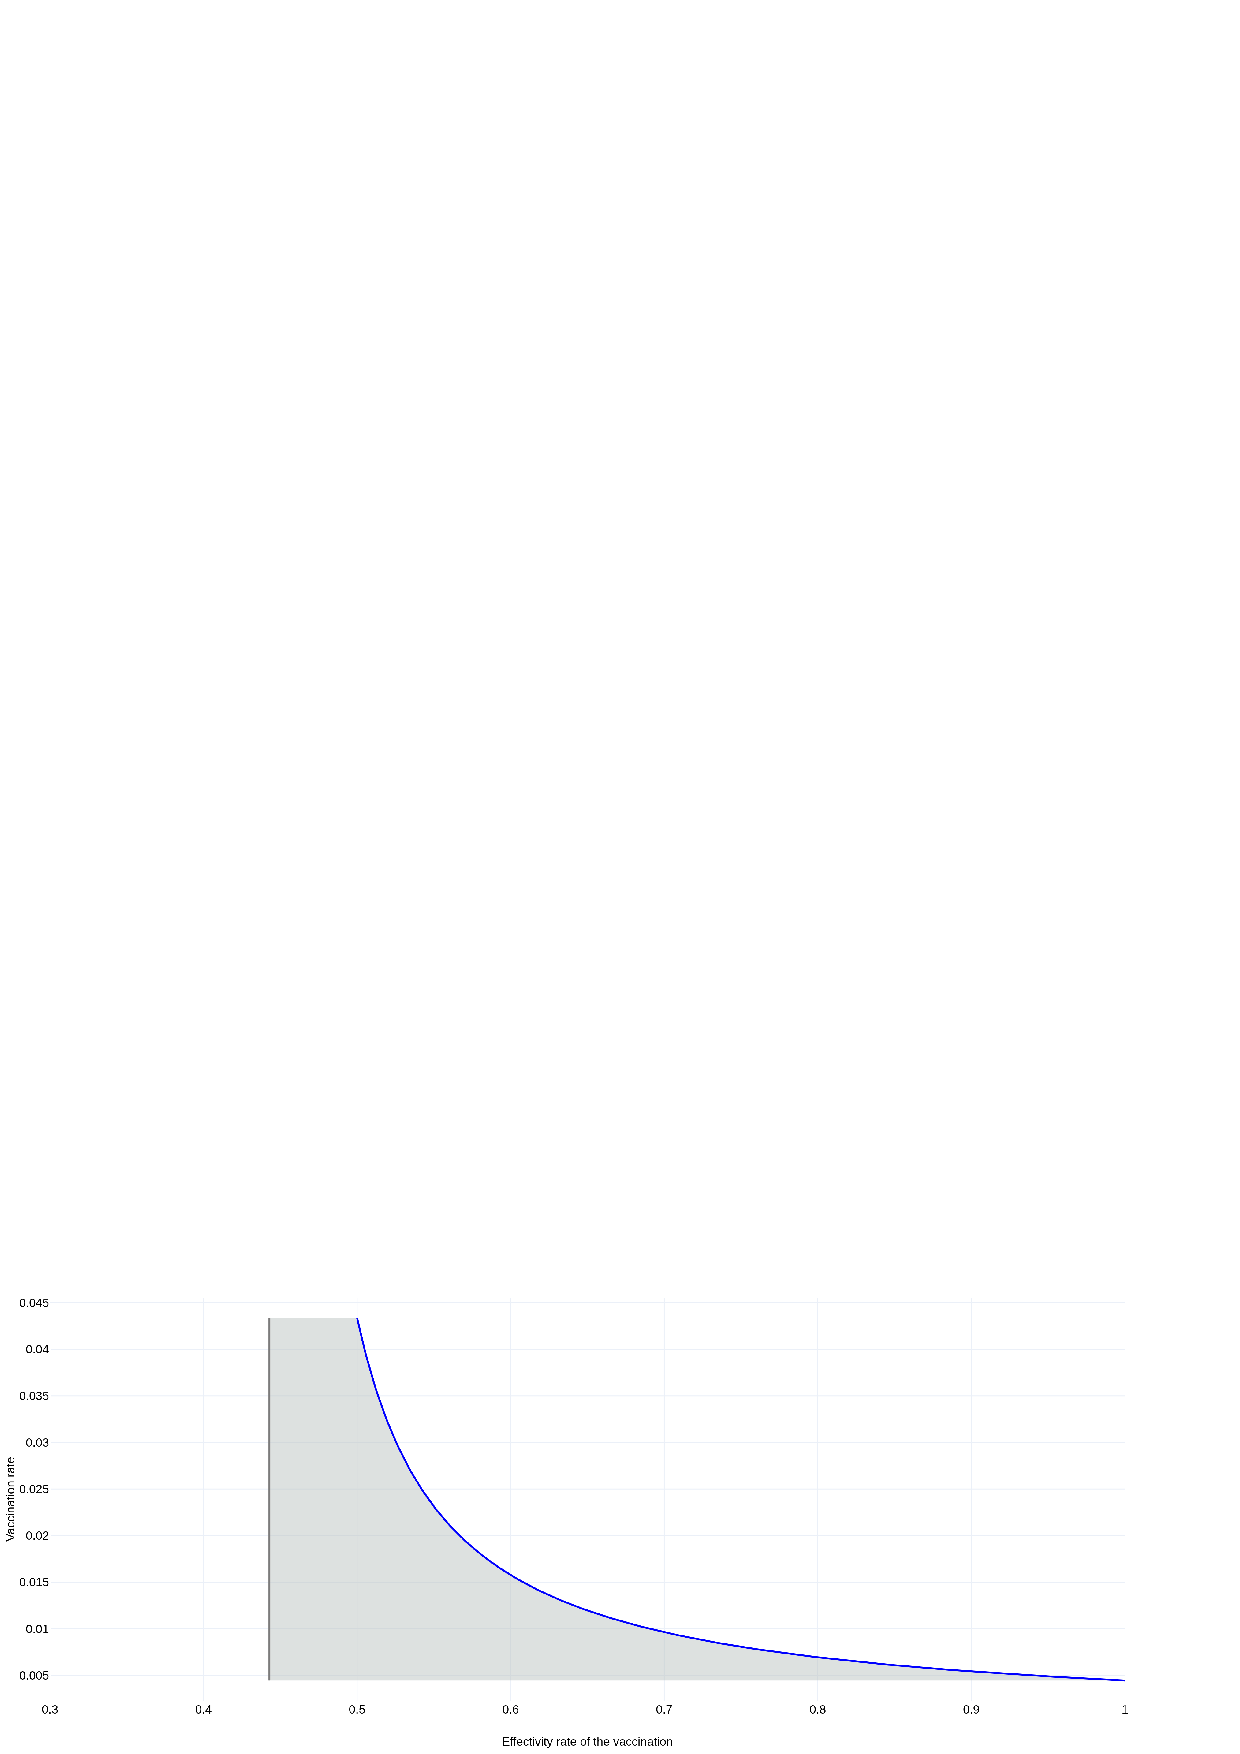
\includegraphics[width=\textwidth]{R0-2D.png}
%  \caption{In the shaded region $ R_V> 1 $ and in the white region $ R_V <1 $.}
%\end{figure}

\begin{figure}[h!]
\centering
\begin{subfigure}[b]{0.45\linewidth}
\includegraphics[width=\linewidth]{R0-2D-A.png}
\caption{$\lambda_V \in (0,1]$ }
\label{figure3A}
\end{subfigure}
\begin{subfigure}[b]{0.45\linewidth}
\includegraphics[width=\linewidth]{R0-2D-B.png}
\caption{$\lambda_V \in (0,0.01]$ }
\label{figure3B}
\end{subfigure}
\caption{In the shaded region $ R_V> 1 $ and in the white region $ R_V <1 $.}
\label{figure3}
\end{figure}

Figure \ref{figure4} shows the regions where it is possible to reduce the value of $ R_V $. In this case, we set all the system parameters, which are given in table \ref{table1} and with $ \delta_V $, $ \epsilon $ and $ \lambda_V $ free.
%\begin{figure}[!h]\label{figure4}
% \includegraphics[width=\textwidth]{R0-3D.png}
%\caption{In the shaded region $ R_V> 1 $ and in the white %region $ R_V <1 $.}
%\end{figure}



\begin{figure}[h!]
\centering
\begin{subfigure}[b]{0.6\linewidth}
\includegraphics[width=\linewidth]{R0-3D-A.png}
\caption{$\lambda_V\in(0,1]$ and $\delta_V\in(0,1]$}
\label{figure4A}
\end{subfigure}
\begin{subfigure}[b]{0.35\linewidth}
\includegraphics[width=\linewidth]{R0-3D-B.png}
\caption{$\lambda_V\in(0,0.01]$ and $\delta_V\in(0,0.01]$}
\label{figure4}
\end{subfigure}
\caption{In the shaded region $ R_V> 1 $ and in the white region $ R_V <1 $.}
\label{figure4B}
\end{figure}

In the next section, the optimal control theory will be applied to propose optimal vaccination dynamics that minimize the number of cases of symptomatic infection and deaths due to the disease.